\newcommand{\bankdistance}{3}
\tikzstyle{bank}=[draw, minimum width=1.5cm, minimum height=1cm, font=\huge,
                  fill=white, rounded corners]
\tikzstyle{op}=[-latex, ultra thick]
\tikzstyle{pline}=[gray, opacity=0.75, thick, -latex]
\newcommand{\plusten}{\textcolor{flatgreen}{+\$10}}
\newcommand{\plustwenty}{\textcolor{flatblue}{+\$20}}
\newcommand{\minusthirty}{\textcolor{flatgreen}{-\$30}}
\newcommand{\minusforty}{\textcolor{flatblue}{-\$40}}

\newcommand{\zigzag}[2]{{
  \newcommand{\banka}{#1}
  \newcommand{\bankb}{#2}
  \draw[gray, op] ($(\banka) + (1.0, 0)$) -- ($(\bankb) + (1.5, 0)$);
  \draw[gray, op] ($(\bankb) + (1.6, 0)$) -- ($(\banka) + (2.0, 0)$);
  \draw[gray, op] ($(\banka) + (2.1, 0)$) -- ($(\bankb) + (2.5, 0)$);
  \draw[gray, op] ($(\bankb) + (2.6, 0)$) -- ($(\banka) + (3.0, 0)$);
}}

\begin{frame}{Replicated Bank Account}
  \begin{center}
    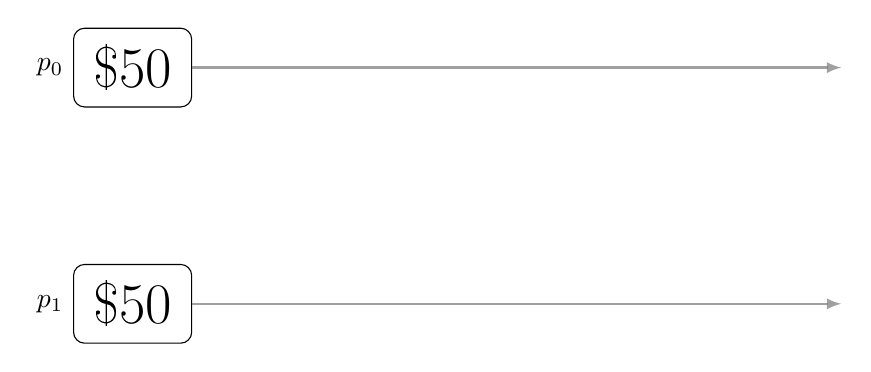
\begin{tikzpicture}
      \node[bank, label=left:{$p_0$}] (a1) at (0, \bankdistance) {\$50};
      \node[bank, label=left:{$p_1$}] (b1) at (0, 0) {\$50};
      \draw[pline] (a1) to (9, \bankdistance);
      \draw[pline] (b1) to (9, 0);
    \end{tikzpicture}
  \end{center}

  \note{%
    We'll begin with an example. \\[12pt]

    Let's say we have an object that we want to replicate. The object can be
    something complex like a database or a key-value store, but to keep things
    simple, let's say we want to replicate a single integer that represents my
    bank account balance. We decide to replicate the integer across two
    machines, replica A and replica B. \\[12pt]

    Users can issue transactions to our replicate object, and every
    transacation is either a deposit or a withdrawal. And, I have one critical
    invariant that I want to maintain at all times. And that invariant is that
    my bank account balance should never be negative. \\[12pt]
  }
\end{frame}

\begin{frame}{Coordinating}
  \begin{center}
    \begin{tikzpicture}
      \node[bank, label=left:{$p_0$}] (a1) at (0, \bankdistance) {\$50};
      \node[bank, label=left:{$p_1$}] (b1) at (0,  0) {\$50};
      \draw[pline] (a1) to (9, \bankdistance);
      \draw[pline] (b1) to (9, 0);
      \draw[op] ($(a1) + (0, +2)$) -- (a1) node[midway, left] {$\plusten$};
      \draw[op] ($(b1) + (0, -2)$) -- (b1) node[midway, left] {$\plustwenty$};
      \pause

      \zigzag{a1}{b1}
      \node[bank] (a2) at (4, \bankdistance) {\$60};
      \node[bank] (b2) at (4, 0) {\$60};
      \draw[op] (a1) to node[above] {$\plusten$} (a2);
      \draw[op] (b1) to node[below] {$\plusten$} (b2);
      \pause

      \zigzag{a2}{b2}
      \node[bank] (a3) at (8, \bankdistance) {\$80};
      \node[bank] (b3) at (8, 0) {\$80};
      \draw[op] (a2) to node[above] {$\plustwenty$} (a3);
      \draw[op] (b2) to node[below] {$\plustwenty$} (b3);
    \end{tikzpicture}
  \end{center}

  \note{%
    One way to replicate our object is by using coordination to implement
    strong consistency. For example, imagine a user issues a deposit of 10
    dollars to replica A, and simultaneously, another user issues a deposit of
    20 dollars to replica B. The two replicas can coordinate and agree on a
    single total order in which to execute the two transactions. Here, the
    replicas deposit 10 dollars and then deposit 20 dollars. Both transactions
    succeed and our invariant is maintained.
  }
\end{frame}

\begin{frame}{Coordinating}
  \begin{center}
    \begin{tikzpicture}
      \node[bank, label=left:{$p_0$}] (a1) at (0, \bankdistance) {\$50};
      \node[bank, label=left:{$p_1$}] (b1) at (0, 0) {\$50};
      \draw[pline] (a1) to (9, \bankdistance);
      \draw[pline] (b1) to (9, 0);
      \draw[op] ($(a1) + (0, +2)$) -- (a1) node[midway, left] {$\minusthirty$};
      \draw[op] ($(b1) + (0, -2)$) -- (b1) node[midway, left] {$\minusforty$};
      \pause

      \zigzag{a1}{b1}
      \node[bank] (a2) at (4, \bankdistance) {\$20};
      \node[bank] (b2) at (4, 0) {\$20};
      \draw[op] (a1) to node[above] {$\minusthirty$} (a2);
      \draw[op] (b1) to node[below] {$\minusthirty$} (b2);
      \pause

      \zigzag{a2}{b2}
      \node[bank] (a3) at (8, \bankdistance) {\$20};
      \node[bank] (b3) at (8, 0) {\$20};
      \draw[op] (a2) to node[above] {$\minusforty$} (a3);
      \draw[op] (b2) to node[below] {$\minusforty$} (b3);
    \end{tikzpicture}
  \end{center}

  \note{%
    Now, consider what happens when two clients issue concurrent withdrawal
    transactions of 30 dollars and 40 dollars. Again, the two replicas
    coordinate. They first withdraw 30 dollars, bringing my bank account
    balance to 20 dollars. They then try to withdraw of 40 dollars but abort
    the transaction because I only have 20 dollars left. Note that even though
    the withdrawal of 40 dollars failed, our invariant is always maintained.
  }
\end{frame}

\begin{frame}{Avoiding Coordination}
  \begin{center}
    \begin{tikzpicture}
      \node[bank, label=left:{$p_0$}] (a1) at (0, \bankdistance) {\$50};
      \node[bank, label=left:{$p_1$}] (b1) at (0, 0) {\$50};
      \draw[pline] (a1) to (9, \bankdistance);
      \draw[pline] (b1) to (9, 0);
      \draw[op] ($(a1) + (0, +2)$) -- (a1) node[midway, left] {$\plusten$};
      \draw[op] ($(b1) + (0, -2)$) -- (b1) node[midway, left] {$\plustwenty$};
      \pause

      \node[bank] (a2) at (4, \bankdistance) {\$60};
      \node[bank] (b2) at (4, 0) {\$70};
      \draw[op] (a1) to node[above] {$\plusten$} (a2);
      \draw[op] (b1) to node[below] {$\plustwenty$} (b2);
      \pause

      \node[bank] (a3) at (8, \bankdistance) {\$80};
      \node[bank] (b3) at (8, 0) {\$80};
      \draw[op] (a2) to node[midway, above] {$\plustwenty$} (a3);
      \draw[op] (b2) to node[midway, below] {$\plusten$} (b3);
      \draw[dashed, op] (a2) -- ($(b3) + (-2, 0)$);
      \draw[dashed, op] (b2) -- ($(a3) + (-2, 0)$);
    \end{tikzpicture}
  \end{center}

  \note{%
    Alternatively, instead of implementing our bank with strong consistency, we
    can implement it with weak consistency and avoid coordination altogether.
    \\[12pt]

    Now, when two clients issue concurrent deposit transactions, the two
    replicas execute the transactions immediately without consulting one
    another. \\[12pt]

    And every once in a while, the two replicas communicate and fill each other
    in on the transactions they missed. Notice that even though we didn't
    perform any coordination, the two replicas never violate the invariant.
    \\[12pt]
  }
\end{frame}

\begin{frame}{Avoiding Coordination}
  \begin{center}
    \begin{tikzpicture}
      \node[bank, label=left:{$p_0$}] (a1) at (0, \bankdistance) {\$50};
      \node[bank, label=left:{$p_1$}] (b1) at (0, 0) {\$50};
      \draw[pline] (a1) to (9, \bankdistance);
      \draw[pline] (b1) to (9, 0);
      \draw[op] ($(a1) + (0, +2)$) -- (a1) node[midway, left] {$\minusthirty$};
      \draw[op] ($(b1) + (0, -2)$) -- (b1) node[midway, left] {$\minusforty$};
      \pause

      \node[bank] (a2) at (4, \bankdistance) {\$20};
      \node[bank] (b2) at (4, 0) {\$10};
      \draw[op] (a1) to node[above] {$\minusthirty$} (a2);
      \draw[op] (b1) to node[below] {$\minusforty$} (b2);
      \pause

      \node[bank] (a3) at (8, \bankdistance) {-\$20};
      \node[bank] (b3) at (8, 0) {-\$20};
      \draw[op] (a2) to node[above] {$\minusforty$} (a3);
      \draw[op] (b2) to node[below] {$\minusthirty$} (b3);
      \draw[dashed, op] (a2) -- ($(b3) + (-2, 0)$);
      \draw[dashed, op] (b2) -- ($(a3) + (-2, 0)$);
    \end{tikzpicture}
  \end{center}

  \note{%
    However, let's look at what happens when two clients issue concurrent
    withdrawals. Both withdrawals are executed locally and both succeed.
    However, when the two replicas exchange transactions with one another, they
    both enter an invariant violating state of negative twenty dollars!
  }
\end{frame}

\begin{frame}
  \Large

  \begin{center}
    \begin{enumerate}
      \item
        Strong consistency preserves the invariant.
      \pause \item
        Deposits don't require coordination.
      \pause \item
        Withdrawals do require coordination.
    \end{enumerate}
  \end{center}

  \note{%
    We can learn a lot from these examples. \\[12pt]

    First, if we implement our bank with strong consistency, we never violate
    our invariant. \\[12pt]

    Second, we can implement deposit transactions without any coordination and
    we're still guaranteed to never violate the invariant. \\[12pt]

    Third, withdrawal transactions, unlike deposit transactions, do require
    coordination to avoid violating the invariant. \\[12pt]

    At a very high level, invariant confluence tries to capture exactly which
    transactions require coordination to maintain invariants and which do not.
    In this example, deposit transactions are invariant confluent and thus do
    not require coordination, while withdrawal transactions not invariant
    confluent and thus do require coordination. \\[12pt]
  }
\end{frame}
